\documentclass[a4paper]{article}
\usepackage{vmargin}
\usepackage{algorithmicx}
\usepackage{algpseudocode}
\usepackage{graphicx}
\usepackage{color}
\usepackage[utf8]{inputenc}
\usepackage{amsmath}
\setpapersize{A4}
\setmargins{2.5cm}       % margen izquierdo
{1.5cm}                        % margen superior
{16.5cm}                      % anchura del texto
{23.42cm}                    % altura del texto
{10pt}                           % altura de los encabezados
{1cm}                           % espacio entre el texto y los encabezados
{0pt}                             % altura del pie de página
{2cm}                           % espacio entre el texto y el pie de página

\begin{document}


\section{Ejercicio 1}
\subsection{Explicación Heurística de búsqueda local1}
Pudimos observar cuando probamos el algoritmo goloso con grafos chicos que la solución no era óptima por poco, y si sólo movíamos algunos nodo a otros conjuntos sí lo era.
De esta forma se nos ocurrió que podíamos mover un nodo a otro conjunto para ver si era mejor la solución.\newline
Así pensamos que la vecindad de una solución podía ser todas las soluciones que difieran en un nodo. 

Para explicar mejor el algoritmo que crea la vencindad utilizaremos el siguiente pseudocódigo, en el cual se usan auxiliares:\newline\

Una \textit{soluci\'on} es un conjunto de conjuntos de nodos, costo\_Solución es un entero

\begin{algorithmic}[1]
\Procedure{CrearVecindad}{\textit{(solución, int costo\_Solución)$\rightarrow$ lista(solución)}}
	\State $\textit{para todos los conjuntos de nodos del conjunto:} $
	\State $\textit{tomar de a uno los nodos dentro del conjunto de nodos}$
	\State $\textit{para todo conjunto distinto de donde tomé el nodo:}$
	\State $\textit{hacer una copia de la solución}$
	\State $\textit{sacar el nodo de la copia}$
	\State $\textit{poner el nodo en el conjunto distinto}$
	\State $\textit{calcular el costo de la copia modificada.}$

	\If{\textit{(el nuevo costo $<$ costo\_Solución)}}
		\State $\textit{armar una tupla (copiaModificada,el nuevo costo)}$
		\State $\textit{guardar la tupla en una lista}$
	\EndIf
\State $\textit{devolver la lista que armé}$

\EndProcedure
\end{algorithmic}
\vspace{0.4cm}
\begin{algorithmic}[1]
\Procedure{ElegirMejor}{\textit{(lista((solución,costo\_Solución)))$\rightarrow$ tupla(solución,costo\_solución)}}
	\State $\textit{Buscar en la lista la túpla que tiene máximo costo\_Solución} $

\EndProcedure
\end{algorithmic}

Grafo es una matriz de $nXn$, donde $n$ es la cantidad de nodos, y en la posición $(i,j)$ está el costo de la arista $(i,j)$
\vspace{0.4cm}
\begin{algorithmic}[1]
\Procedure{K\-PMP\_Busqueda\_Local}{\textit{(solución solu, entero costo\_solu ,entero K)$\rightarrow$ tupla(solución)}}
	\State $\textit{lista(solución) lsolu= crearVecindad(solu,costo\_solu)} $
	\State $\textit{devolver eslegirMejor(lsolu)} $
	
\EndProcedure
\end{algorithmic}
\vspace{0.4cm}
En el pseudocódigo de K\-PMP\_Busqueda\_Local la entrada es una solución, y dos enteros, pero en la implementación la entrada es un grafo (matriz) y un entero. Esto es porque dentro del algoritmo aplicabamos la implementación de la heurística golosa para obtener la solución a la que ibamos a buscar los vecinos o sólo metíamos todos los nodos en un conjunto dejando los otros vacíos. De esta manera podíamos experimentar sin tener que darle a la entrada una solución y nos resultó más comodo. 



\subsection{Complejidad Heurística de búsqueda local1}

Para calcular la complejidad de CrearVecindad vamos a calcular la complejidad de los "auxiliares" que utiliza.\newline
En CrearVecindad tenemos: \newline
Línea 2 : La cantidad de conjuntos es $k$, entonces tengo costo $k$, porque usamos vector que tiene costo constante para el acceso(\textit{http://www.cplusplus.com/reference/vector/vector/operator\%5B\%5D/}).\newline
Línea 3: Recorrer los nodos dentro del conjunto en peor caso es $n$, cantidad de nodos y asumiendo que todos los conjuntos tienen esa cantidad. Para representar los conjuntos utilizamos vector,como el acceso es $O(constante)$(\textit{http://www.cplusplus.com/reference/vector/vector/operator\%5B\%5D/}),entonces tengo costo n.\newline
Línea 4: Lo mismo que en línea 2, sólo que ahora tengo una comparación (es o no el nodo que saqué) que tiene costo 1. Entonces tengo costo $k$.\newline
Línea 5: Tengo $k$ conjuntos con $n$ nodos, con lo cual tengo costo $n*k$, también porque usamos vector y hacer una copia tiene costo la cantidad de elemntos(\textit{http://www.cplusplus.com/reference/vector/vector/operator=/}).\newline
Línea 6: Buscarlo en el conjunto tiene costo $n$(por usar vector), luego borarlo tiene costo $1$(tiene costo la cantidad de elementos por usar un vector \textit{http://www.cplusplus.com/reference/vector/vector/erase/}), con lo cual tengo costo $n+1$.\newline
Línea 7: Agregarlo en el conjunto a modificar tiene costo 1\newline(\textit{www.cplusplus.com/reference/vector/vector/push\_back/}).\newline
Línea 8: Recorro cada uno de los conjuntos (costo $k$) y 
calculo "las aristas que se generan dentro" para sumarlas (en peor caso tengo costo $n^{2}$ todos los nodos con todos). Entonces tengo costo $k*n^{2}$. \newline
Línea 9: Una comparación de números, costo 1.\newline
Línea 10 y 11: Armar la túpla y meterla en una lista tiene costo 1, porque usamos un vector para representar la lista, usando push\_back que tiene costo constante. \newline

Como tenemos muchos "fors" anidados, el costo total es la multiplicación del costo de cada "for"
Con lo cual la complejidad de $CrearVecindad$ es $k^{3}*n^{3}$ .


ElegirMejor tiene costo la cantidad de elemenos que hay en la lista:
Para cada conjunto, cuya cantidad es $k$, voy a tomar cada uno de los elementos, en peor caso tengo $n$, y los voy a meter en cada uno de los conjuntos.
Con lo cual en peor caso son $k^{2}*n$ elementos dentro de la lista, y como suamos vector para representarla tenemos costo la cantidad de elementos, con lo cual tengo costo $k^{2}*n$

Finalmente el costo de \textit{K\-PMP\_Busqueda\_Local} es la suma del costo de $CrearVecindad$ y $ElejirMejor$,ya que devolver la tupla tiene costo 1 y la forma de crear la solución no es relevante porque , entonces tenemos $O(k^{3}*n^{3})$

\subsection{Explicación Heurística de búsqueda local2}

Para la resoluci\'on se cuenta inicialmente con una K-partici\'on con sus elementos (nodos) distribuidos de alguna forma, la llamaremos $solucion$. Lo que se va a proceder a hacer es tratar de mejorar el peso total de esta K-partici\'on (con peso total nos referimos a la suma de los pesos de todos los conjuntos de dicha partici\'on). Reubicando sus nodos de manera que se minimice dicho peso.
Para esto y siguiendo la idea de b\'usqueda local se construir\'an varias posibles soluciones, vecinos, y nos quedaremos con el mejor de ellos (el mejor es aquel, cuyo peso total sea el m\'inimo de entre los vecinos que constituyen la vecindad).  
Para la resoluci\'on, empezaremos tomando al primero de los conjuntos  que constituyen a $solucion$. Una vez tomado, se trabajara con los nodos dentro del mismo y de a par, siempre que estos sean adyacentes. Si no hay nodos adyacentes en el conjunto, entonces se devolver\'a como solucion y vecino, a $solucion$ (no se producen cambios). En caso de existir al menos un  par de nodos adyacentes. Evaluaremos el peso que se genera entre la arista que une a este par y el peso de las aristas a los nodos adyacentes dentro del conjunto actual, $peso\_combinacion$. Calculado este \'ultimo peso, nos quedaremos con aquel cuyo valor es m\'aximo, $mayor\_peso$. Una vez hallado este par de nodos, a los que llamaremos a uno $nodo\_A$ y otro $nodo\_B$, crearemos otra K-partici\'on, $nuevo\_vecino$. El mismo sera una copia de la $solucion$ actual, solo que no contara con los nodos denominados $nodo\_A$ y $nodo\_B$.  Y lo que se va a proceder a hacer es a reubicar a ambos nodos en aquel o aquellos conjuntos tal que el peso final de $nuevo\_vecino$ sea m\'inimo. Y tendremos una posible soluci\'on. Finalizado esto, se procede a operar de la misma manera pero, ahora trabajando con el siguiente conjunto. De esta forma vamos a obtener un nuevo vecino. Luego de haber trabajado con los k conjuntos elegiremos a aquel vecino de todos los formados cuyo peso total sea el m\'inimo. Como $solucion$ es hasta el momento la soluci\'on para el problema, se comparara si el peso del vecino elegido es menor que este. Si no lo es, no se pudo obtener una mejor ubicaci\'on  que la que ya se tenia para los nodos y se finaliza el algoritmo siendo $solucion$ la solucion a nuestro problema. En caso de serlo $solucion$ pasara a ser el vecino seleccionado. Y se comenzara a ejecutar nuevamente lo propuesto inicialmente, pero ahora con la K-partici\'on $solucion$ modificada. Para poder seguirla optimizando.


\vspace{0.4cm}
\begin{algorithmic}[1]
\Procedure{vecindad2}{\textit{..solucion, total de conjuntos,..}}       
        \State $suma\_solucion \gets \textit{sumar el peso de la solucion}$
        \If {(\textit{solucion no usa los k conjuntos})}
        		\State $ \textit{agregar conjuntos restantes vacios a solucion} $
        \EndIf
        \State vecino\_solucion $\gets \textit{crear una nueva k\_particion}$     
        \State posible\_solucion $\gets -1$
		\While{(\textit{se pueda mejorar suma\_solucion})}    
        		\For{ i= 1,...,$total$ $de$ $conjuntos$}
                \If{$(\textit{solucion[i] tiene mas de un nodo})$}
					\State nuevo\_vecino $\gets \textit{crear una nueva k\_particion}$                              
                		\State $peso\_vecino \gets \textit{ crear\_vecino(...,i, ,solucion, vecino\_actual,..)} $ 
                \EndIf
                \If{$(peso\_vecino < posible\_solucion$ $o$ $posible\_solucion == -1)$}
                		\State posible\_solucion $\gets peso\_vecino$
                		\State vecino\_solucion $\gets nuevo\_vecino$
                \EndIf     
			\EndFor   
			\If {$(posible\_solucion < suma\_solucion)$}
				\State suma\_solucion $ \gets posible\_solucion$
				\State solucion $ \gets vecino\_solucion$
				\State posible\_solucion $\gets -1$
			\Else
				\State $return$ $solucion$
			\EndIf   
        \EndWhile            
        \State Return solucion
\EndProcedure
\end{algorithmic}

\vspace{0.4cm}
\begin{algorithmic}[1]
\Procedure{crear\_vecino}{$..i,solucion, vecino\_actual..$}
        \For {\textit{cada combinacion entre par de nodos adyacente dentro de solucion[i]}}
				\State nodo\_A $\gets \textit{tomar un nodo de solucion[i]}$ 
				\State nodo\_B $\gets \textit{tomar un nodo adyacente a nodo\_A en solucion[i]} $              
                \State peso\_combinacion $\gets \textit{sumar el peso de la arista entre el nodo\_A y el nodo\_B y el peso de las aristas}  \newline \textit{de los nodos adyacentes a nodo\_A y nodo\_B dentro de solucion[i]}$
			    \State mayor\_peso $\gets$ $el$ $mayor$ $peso\_combinacion $
			    \State separo\_A $\gets$ $nodo\_A$ $con$ $mayor$ $peso\_combinacion$
			    \State separo\_B $\gets$ $nodo\_B$ $con$ $mayor$ $peso\_combinacion$     
		\EndFor	         
         \State nuevo\_vecino  $\gets solucion$ 
         \State \textit{sacar a los nodos separo\_A y separo\_B del conjunto nuevo\_vecino[i]}   
         \State \textit{ubicar a los nodos separo\_A y separo\_B entre los conjuntos de nuevo\_vecino de manera de minimizar el peso total} 
         \State \textit{return peso total de nuevo\_vecino}
\EndProcedure
\end{algorithmic}
\vspace{0.4cm}

 \textit {tanto solucion[i] como nuevo\_vecino[i] hacen referencia al i-esimo conjunto de cada K-partici\'on. Con los conjuntos enumerados de 1 al total de conjuntos.}
 
\subsection{Complejidad Heurística de búsqueda local2}
 
Para representar la K-partici\'on $solucion$, se utilizo un vector de tuplas. donde la segunda componente emula un conjunto, por medio de un vector de int, y la primera a la suma del peso de dicho conjunto. 
El algoritmo cuenta con dos funciones principales que son las mencionadas $vecindad2$ y $crear$ $vecino$, como el mismo se ejecuta hasta que ya no se pueda mejorar al vector $solucion$. Analizaremos la complejidad de cada iteraci\'on.  \newline \newline
1) Complejidad de $vecindad2$:\newline
a) Como se trabaja a partir de una soluci\'on\'on dada, la misma quiz\'as no utiliza la cantidad total de conjuntos con que dispone. Entonces se procede a completar al vector $solucion$ con las tuplas restantes. O(k)\newline
b) Se crear un vector vac\'io, que almacenara al mejor de los vecinos. O(1) y se comienza con las mencionadas iteraciones. \newline
c)Por cada conjunto de $solucion$ se llama a la funci\'on crear vecino. Es decir se la llama k veces (siendo k la cantidad de conjuntos). \newline
d) Cada vez que se obtiene un $nuevo\_vecino$ y su peso, se verifica si es menor que el peso de los anteriores vecinos o si es el primer vecino creado. En caso de serlo se guarda este peso 0(1) y tambien a $nuevo\_vecino$ en $vecino\_solucion$ O(k+n) (n cantidad de nodos en total). Como esto se realiza a lo sumo para todos los conjuntos tenemos O(k*(k+n))\newline
e) Finalizada estas iteraciones, se verifica si el peso de $vecino\_solucion$ es menor que el peso de $solucion$ en caso de serlo se guarda el peso y se reemplaza a $solucion$ O(k+n). Y se vuelve a realizar una nueva iteraci\'on.\newline \newline 
2) Complejidad de $Crear$ $vecino$: \newline
a) Esta funci\'on comienza por buscar a los pares de nodos que sean adyacentes y calculando su $peso\_combinacion$. Para obtener todas las combinaciones se emplearon dos for anidados, el primero de ellos va desde 1 al total de nodos en el conjunto que se esta utilizando, denominaremos t a esta cantidad con 0 $<=$ t $<$ n. El segundo comienza desde el siguiente nodo que se este utilizando en el primero de los for hasta t. De esta forma obtenemos todas las combinaciones. Pero, por cada una hay que sumar el peso de la arista que los une y el peso de sus adyacentes. Para calcular este \'ultimo, se vuelve a recorrer a todos los nodos y si son adyacentes se suma el peso de la arista. El mismo se encuentra en una matriz a la que podemos acceder en O(1). De esta manera se realizan, para generalizar, dos for de 1 hasta t. y en cada iteracion una suma de t elementos en total O($t^{3}$).
Comparando cada $peso\_combinacion$ realizado para guardarnos el m\'aximo O(1). \newline
b) Procedemos a copiar al vector $solucion$ a $nuevo\_vecino$ O(k + n), y a retirar del i-esimo conjunto (i-esima tupla) de este \'ultimo vector a $nodo\_A$ y $nodo\_B$ O(t).  Y se actualiza la primer componente con la suma correspondiente. Que es la cantidad de aristas, en el peor de los casos O($t^{2}$).  \newline
c) Para encontrar la mejor ubicaci\'on del par de nodos es necesario ver todos las combinaciones con los k conjuntos y ubicarlo donde el peso total generado sea el m\'inimo que con alguna otra combinaci\'on. Para representar esto, se crearan dos vectores de longitud k (cada posici\'on  hace referencia a un conjunto de $nuevo\_vecino$). El primero posee en cada posici\'on el peso que se adiciona al meter al $nodo\_A$ en cada conjunto y el segundo al adicionado por insertar a $nodo\_B$. De esta manera, se busca la combinacion de estos vectores donde el valor de la posici\'on de uno mas la del otro sea la m\'inima O($k^{2}$). Y se guarda las posiciones elegidas. \newline
d) Por \'ultimo se inserta al par de nodos en las posiciones elegidas dentro de $nuevo\_vecino$ y se calcula el peso total de este vector O(k)\newline \newline
El costo total de esta funci\'on es por lo tanto O($t^{3}$) + O(k + n) + O(t) + O($t^{2}$)+ O($k^{2}$) + O(k) = O($t^{3}$) + O($k^{2}$) + O(n) \newline t es como m\'aximo igual a n. Acotamos t por n y obtenemos: \newline O($n^{3}$ + $k^{2}$) \newline
Pero esta funci\'on como se menciono en el punto 1.c es llamada k veces entonces tenemos: \newline O(k*($n^{3}$ + $k^{2}$)) \newline
Agregando los costos de la funci\'on $vecindad2$ tenemos en total: \newline 
O(k) + O(k*($n^{3}$ + $k^{2}$)) + O(k*(k + n)) + O(k + n) = O(k*$n^{3}$ + $k^{3}$) 


\section{Experimentación de las heurísticas locales}
Primero vamos a corroborar empíricamente que las complejidades que calculamos teóricamente son correctas. Para esto generamos grafos completos de 1 a 100 nodos, con los pesos de las aristas un número aleatorio entre 0 y 50(en $\Re$).Luego aplicamos las heuristicas locales 5 veces, calculamos promedio, máximo y mínimo tiempo  de las 5 veces por cada instancia. Obtuvimos los siguientes gráficos:\newline
\textbf{\textit{Para la primera heurísica local:}\newline}

Aplicamos el algoritmo con $k=10$ y las instancias de grafos mencionadas anteriormente.\newline
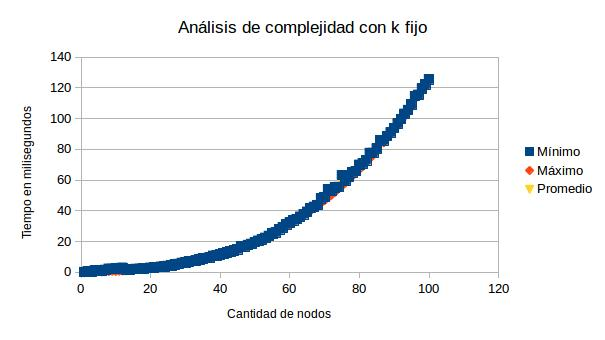
\includegraphics[width=\textwidth,height=\textheight,keepaspectratio
]{local1Kfijo.jpg}
\begin {flushleft}
\textbf{Figure 1:} Con este grafo no podemos ver si realmente es $O((k^{3}*n^{2})+ (k^{2}*n^{3}))$, para poder evidenciarlo mejor vamos a dividir el tiempo por $O((k^{3}*n^{2})+ (k^{2}*n^{3}))$ y deberíamos obtener una constante. \newline
Además podemos comentar que no hay diferencia notable entre el máximo, mínimo y promedio.
\end{flushleft}

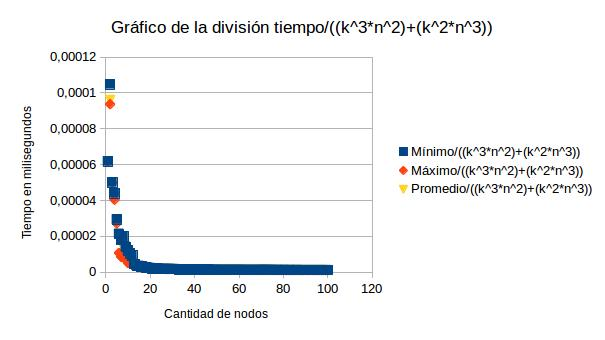
\includegraphics[width=\textwidth,height=\textheight,keepaspectratio
]{local1KfijoConstante.jpg}
\begin {flushleft}
\textbf{Figure 2:} Vemos que tiende a una constante, pero esta es 0 a simple vista, y si realmente tiende a 0 no es nada bueno, veamos que la constante es distinta a 0. Para esto vamos a hacer "zoom" en 0 y ver que las líneas no están ahí.\newline
\end{flushleft}

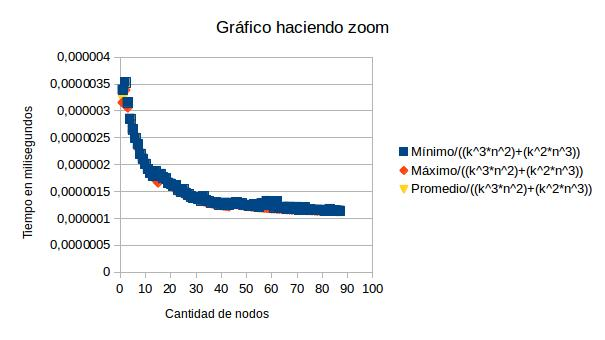
\includegraphics[width=\textwidth,height=\textheight,keepaspectratio
]{local1KfijoConstanteZoom.jpg}
\begin {flushleft}
\textbf{Figure 3:} Podemos ver así que la constante a la que tiende está entre o,000002 y 0,000005 que es distinta de 0. Con esto podemos concluir que la complejidad explicada teóricamente, empíricamente también lo es.
\end{flushleft}
\vspace{0.4cm}


\textbf{\textit{Para la segunda heurísica local:}\newline}

Aplicamos el algoritmo con $k=10$ y las instancias de grafos mencionadas anteriormente.\newline
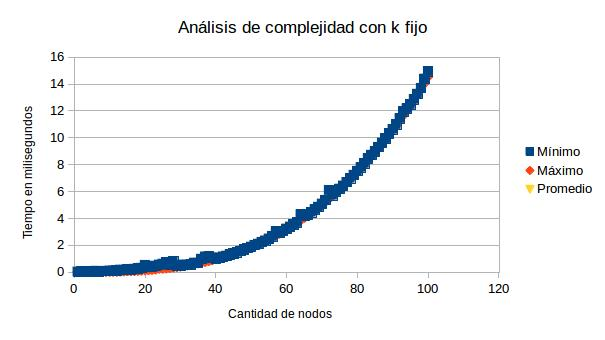
\includegraphics[width=\textwidth,height=\textheight,keepaspectratio
]{local2Kfijo.jpg}
\begin {flushleft}
\textbf{Figure 1:} Con este grafo no podemos si realmente es $O(k^{3}+k*n^{3})$, para poder evidenciarlo mejor vamos a dividir el tiempo/$(k^{3}+k*n^{3})$ y deberíamos obtener una constante. \newline
Además podemos comentar que no hay diferencia notable entre el máximo, mínimo y promedio.
\end{flushleft}

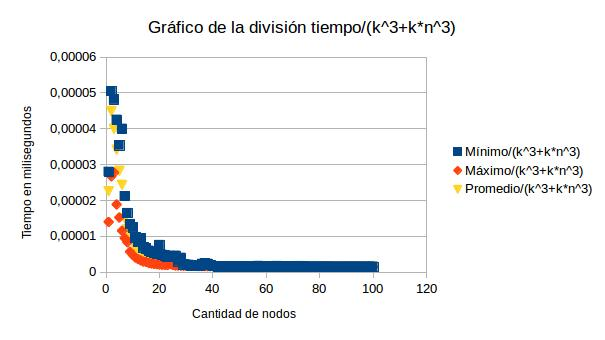
\includegraphics[width=\textwidth,height=\textheight,keepaspectratio
]{local2KfijoConstante.jpg}
\begin {flushleft}
\textbf{Figure 2:} Vemos que tiende a una constante, pero esta es 0 a simple vista, y si realmente tiende a 0 no es nada bueno, veamos que la constante es distinta a 0. Para esto vamos a hacer "zoom" en 0 y ver que las líneas no están ahí.\newline
Aquí si se puede ver la diferencia entre promedio,máximo y mínimo pero es despreciable.
\end{flushleft}

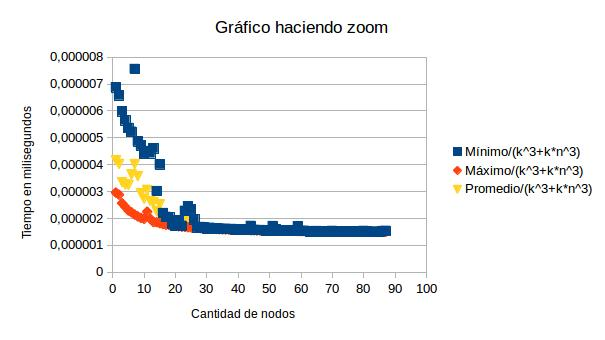
\includegraphics[width=\textwidth,height=\textheight,keepaspectratio
]{local2KfijoConstanteZoom.jpg}
\begin {flushleft}
\textbf{Figure 3:} Podemos ver así que la constante a la que tiene está entre o,000002 y 0,000001 que es distinta de 0. Con esto podemos concluir que la complejidad explicada teóricamente, empíricamente también lo es.
\end{flushleft}
\vspace{0.4cm}
\textbf{\textit{Experimentación para ambas locales:}\newline}
Para experimentar usamos gráfos aleatoizados, es decir, la forma que tiene el grafo es aleatoria al igual que el peso de las aristas. Generamos 50 instancias de estos grafos con aristas en un rango de 0 a 50(en $\Re$) y la cantidad de nodos en un rango de 1 a 50 y otras 50 con el mismo rango de aristas pero con 50 nodos. 
Luego ejecutamos las heurísticas locales 5 veces para cada una de las 50 instancias, quedándonos con el promedio del tiempo de las 5 para cada instancia. Así obtuvimos los tiempos con los que realizamos los siguientes gráficos.\newline


Notamos como $local1$ a la aplicación del algoritmo de la primera vecindad, donde la solución que recibe, es meter todos los nodos en un conjunto y dejar los otros vacíos. Lo mismo para $local2$ pero aplicando el algoritmo de la segunda vecindad. Por otra parte $local1Golo$ tomo como solución la aplicación del algoritmo goloso y luego a la solución modificada le aplica la primera vecindad, lo mismo para $local2Golo$ pero aplicando la segunda vecindad. Además cabe aclarar que los tiempos no son de una iteración del algoritmo, sino, de toda la ejecución.\newline

Para $k$ aleatorio en un rango de 2 a $i$, donde $i$ es la cantidad de nodos del grafo sobre el que se aplica el algoritmo.Y las instancias de grafos son los que varían en la cantidad de nodos:

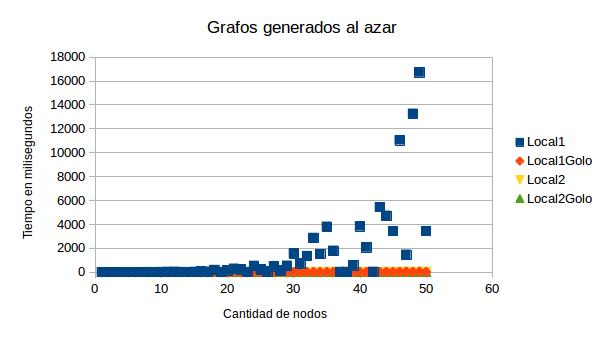
\includegraphics[width=\textwidth,height=\textheight,keepaspectratio
]{KaleN1-50.jpg}
\begin {flushleft}
\textbf{Figure 4:} Vemos claramente que $local1$ tarda mucho más en comparación con las demás que tardan práctiamente lo mismo a simple vista, veamos que pasa cuando hacemos "zoom" para ver los tiempos más chicos.
\end{flushleft}


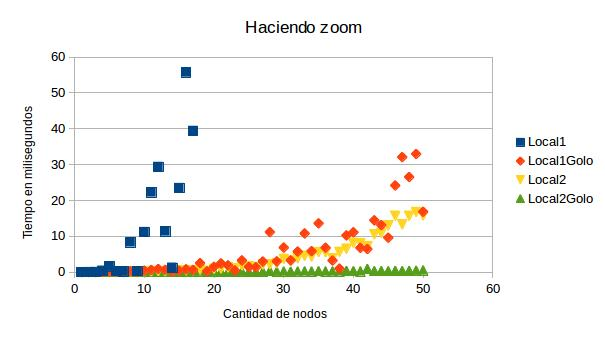
\includegraphics[width=\textwidth,height=\textheight,keepaspectratio
]{KaleN1-50Zoom.jpg}
\begin {flushleft}
\textbf{Figure 5:} Se puede observar que local2Golo es la más rápida, entre local1Golo y local2 hay altos y bajos, pero pareciera que local1Golo se hace más lenta cuando n aumenta.
\end{flushleft}

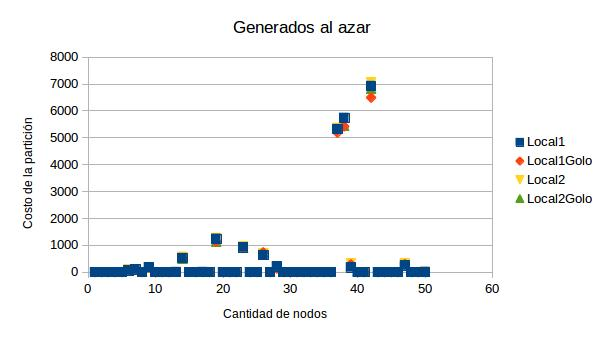
\includegraphics[width=\textwidth,height=\textheight,keepaspectratio
]{KaleN1-50Suma.jpg}
\begin {flushleft}
\textbf{Figure 6:} En cuanto al costo de la partición se puede ver que son prácticamente iguales, para todos los algoritmos. En los grafos anteriores vimos que $local1$ tarde notablemente mucho más que los otros, y acá podemos ver que el resultado es prácticamente el mismo. Entonces no vale la pena invertir tanto tiempo en $local1$ si con los otros podemos obtener casi lo mismo en poco tiempo, en comparación.
\end{flushleft}

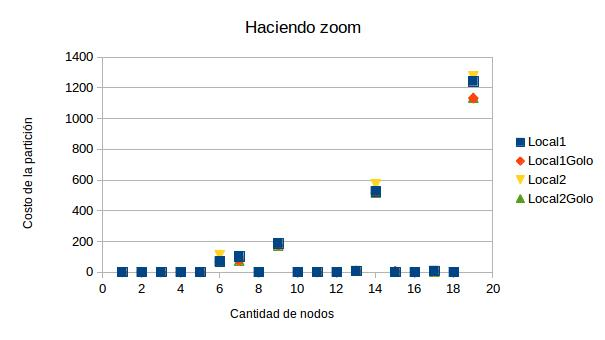
\includegraphics[width=\textwidth,height=\textheight,keepaspectratio
]{KaleN1-50SumaZoom.jpg}
\begin {flushleft}
\textbf{Figure 7:} Hicimos algo de "zoom" para ver si realmente la diferencia era muy poca, y se ve claramente que la mayoría de las veces es casi lo mismo.
\end{flushleft}

Para $k=3$, y las instancias de grafos son los que varían en la cantidad de nodos:


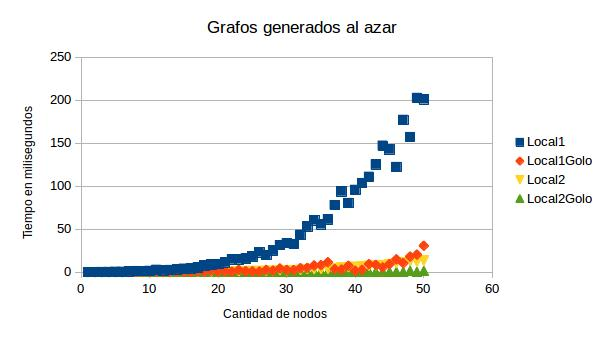
\includegraphics[width=\textwidth,height=\textheight,keepaspectratio
]{k3n1-50.jpg}
\begin {flushleft}
\textbf{Figure 8:} No podemos decir más que pasa lo mismo que en las instancias anteriores, $local1$ es más lenta que todas las demás en comparación. Cabe mencionar que al ser k fijo y no aleatorio como antes, el tiempo de ejecución es mucho menor.
\end{flushleft}

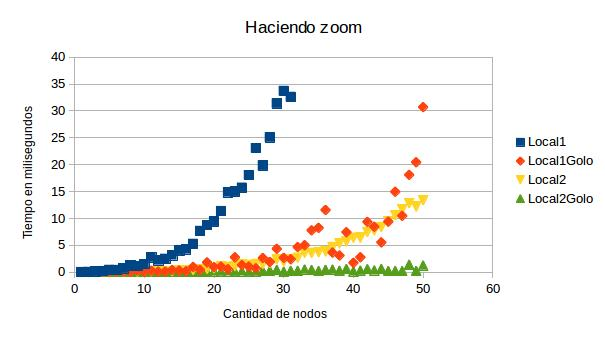
\includegraphics[width=\textwidth,height=\textheight,keepaspectratio
]{k3n1-50Zoom.jpg}
\begin {flushleft}
\textbf{Figure 9:} Vemos que $local1Golo$ y $local2$ tienen un intercambio de "mejor" al principio, pero luego de $n=45$ la mejor es $local2$.
\end{flushleft}

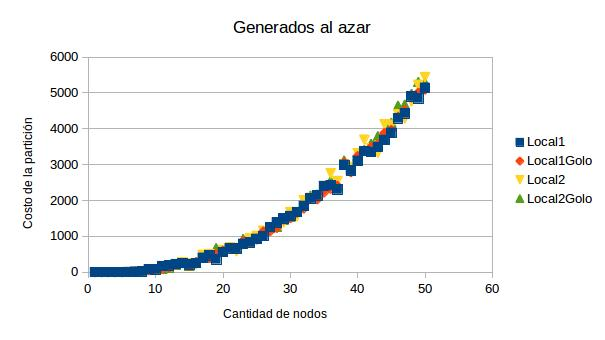
\includegraphics[width=\textwidth,height=\textheight,keepaspectratio
]{k3n1-50Suma.jpg}
\begin {flushleft}
\textbf{Figure 10:} Como era de esperar el costo de la partición aumenta cuando n aumenta, porque k es fijo, entonces "hay menos lugar" para poner los nodos sin que estos generen aristas que suman al costo de la partición.
\end{flushleft}

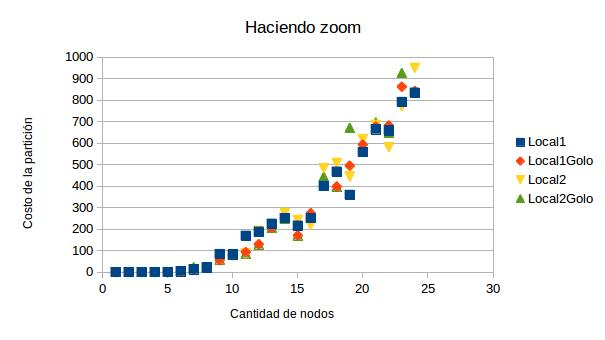
\includegraphics[width=\textwidth,height=\textheight,keepaspectratio
]{k3n1-50SumaZoom.jpg}
\begin {flushleft}
\textbf{Figure 11:} Algoritmos son más eficientes, es decir, dan resultados con menos costo. La diferencia entre ellos es casi despreciable cuando n es chico pero a medida que n aumenta se hace más notable la brecha entre ellos.
\end{flushleft}

Finalmente la última experimentación es con $k$ en el rango de 1 a 50 y los grafos con las intancias con n fijo:\newline

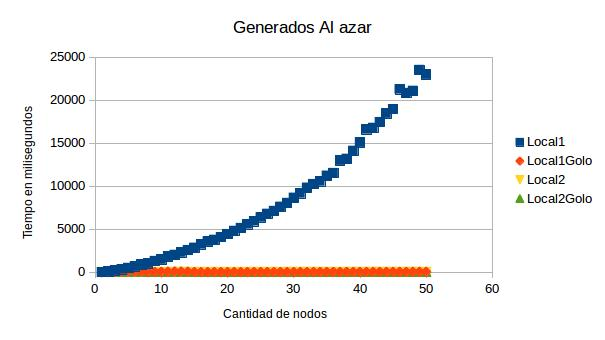
\includegraphics[width=\textwidth,height=\textheight,keepaspectratio
]{N50K1-50.jpg}
\begin {flushleft}
\textbf{Figure 12:} Como era de esperar aumenta en función de k, claramente $local1$ es la "perdedora" en toda esta experimentación. Las demás locales son iguales a simple vista, veamos un poco más los tiempos menores.
\end{flushleft}

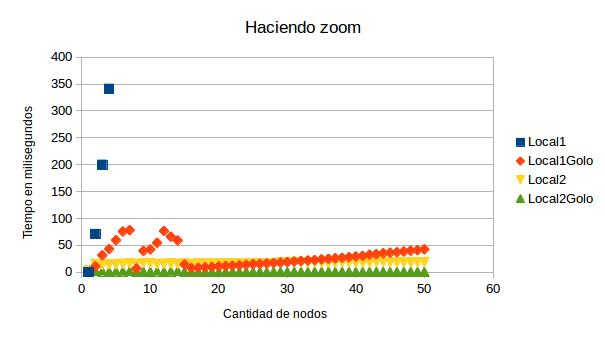
\includegraphics[width=\textwidth,height=\textheight,keepaspectratio
]{N50K1-50Zoom.jpg}
\begin {flushleft}
\textbf{Figure 13:} Si bien en el grafo anterior parecía que todas menos $local1$ eran iguales acá podemos ver que no es así.
\end{flushleft}

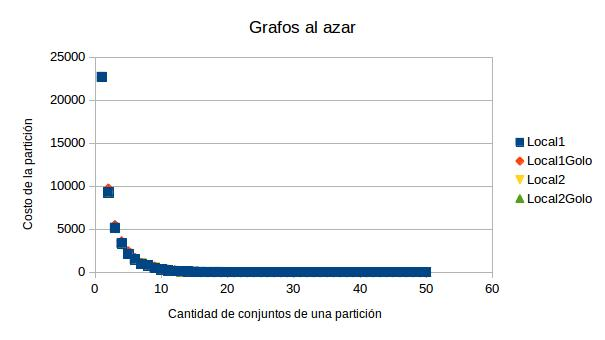
\includegraphics[width=\textwidth,height=\textheight,keepaspectratio
]{N50K1-50Suma.jpg}
\begin {flushleft}
\textbf{Figure 14:} Si la cantidad de nodos es fija, y aumento la cantidad de conjuntos para separarlos, se ve claramente que tengo más posibilidades para ponerlos sin que se generen aristas en los conjuntos. Este grafo deja en evidencia que esto es así, pero veamos que sucede en el medio, cuando no tengo ni pocos ni muchos conjuntos($k$).
\end{flushleft}

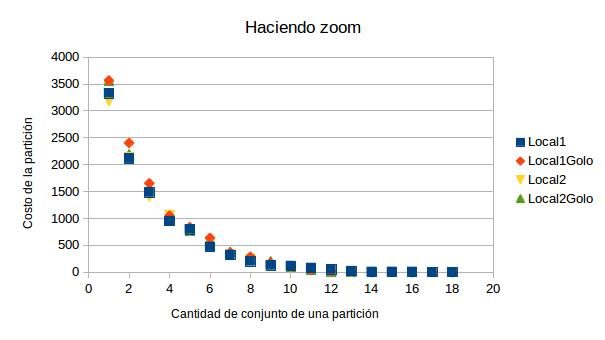
\includegraphics[width=\textwidth,height=\textheight,keepaspectratio
]{N50K1-50SumaZoom.jpg}
\begin {flushleft}
\textbf{Figure 15:} Para todas las locales los resultados son casiiguales, e iguales al "final"
\end{flushleft}

En conclusión como vimos a lo largo de toda la experimentación $local1$ es la que más tarda en comparación con las otras 3 y para colmo esta inversión en tiempo no da una solución mejor. Entre las otras no hay una diferencia drástica en cuanto a tiempo y menos en costo, porque la siempre estaban "pegadas".\newline
En fin, no usaríamos $local1$ teníendo alguna de las otras 3, y como mejor elegimos a la $local2Golo$ que fue la mejor en tiempo en los 3 experimentos que realizamos.
 
\end{document}